\chapter{二元函数、极限与连续}

本章讨论二元函数微积分最基本的概念:二元函数、极限、连续。

如无特殊说明,本章以二元函数为例进行定义和讨论。
好处是方便作图说明,较为直观。
二元数量值函数:
\[
z=f\left( \boldsymbol{p} \right) \quad \boldsymbol{p}=\left( \begin{array}{c}
	x\\
	y\\
\end{array} \right) \in \mathbb{R} ^2
\]
在几何上可以用三维空间的曲面和曲线表示。如$x,y$无约束,则描述一个三维曲面,如$x,y$有约束关系,则描述一条三维曲线。

本章要点:
\begin{itemize}
    \item 极限。
    \item 连续。
\end{itemize}

~

\newpage
\section{邻域、区域与函数}

本节介绍二元函数微积分的基础概念。

本节要点:
\begin{itemize}
    \item 掌握邻域的概念;
    \item 理解点集的各个概念;
    \item 熟悉二元函数的定义。
\end{itemize}

%============================================================
\subsection{邻域}

\begin{definition}[邻域]
设矢量$\boldsymbol{p}_0\in \mathbb{R} ^2$,对于$\delta >0$,所有符合$\left\| \boldsymbol{p}-\boldsymbol{p}_0 \right\| <\delta $的矢量$\boldsymbol{p}$的集合,称为{\bf $\boldsymbol{p}_0$的$\delta $邻域},记作$U\left( \boldsymbol{p}_0,\delta \right) $,若点$\boldsymbol{p}_0$不包含在邻域内,称该集合为{\bf $\boldsymbol{p}_0$的空心$\delta $邻域},记作$U\left( \boldsymbol{\hat{p}}_0,\delta \right) $,即:
\begin{align*}
&U\left( \boldsymbol{p}_0,\delta \right) :=\left\{ \boldsymbol{p}\in \mathbb{R} ^2 \middle| \left\| \boldsymbol{p}-\boldsymbol{p}_0 \right\| <\delta \right\} \\
&U\left( \boldsymbol{\hat{p}}_0,\delta \right) :=\left\{ \boldsymbol{p}\in \mathbb{R} ^2 \middle| 0<\left\| \boldsymbol{p}-\boldsymbol{p}_0 \right\| <\delta \right\}
\end{align*}
\end{definition}

邻域的定义和一元函数中的概念一样,定义了以某点为中心的一个范围。
几何上,二元函数的邻域是一个“面”,三元函数中是一个“球”。

%============================================================
\subsection{点、集和区域}

\begin{definition}

设点集$D$中的点$\boldsymbol{p}_0$,若存在$\boldsymbol{p}_0$的某个邻域$U\left( \boldsymbol{p}_0,\delta \right) \subset D$,称点$\boldsymbol{p}_0$为$D$的{\bf 内点}。
如果点$\boldsymbol{p}_0$的任一邻域中,既有属于$D$的点,也有不属于$D$的点,称点$\boldsymbol{p}_0$为$D$的{\bf 边界点}。
内点和边界点又称为{\bf 聚点}。
$D$的边界点的集合称为$D$的{\bf 边界}。
注意,边界点既可以属于$D$(闭集)也可以不属于$D$(开集)。
反之,设点集$D$外的点$\boldsymbol{p}_0$,若存在$\boldsymbol{p}_0$的某个邻域$U\left( \boldsymbol{p}_0,\delta \right) \cap D=\oslash $,称点$\boldsymbol{p}_0$为$D$的{\bf 外点}。
\begin{figure}[h]
\centering
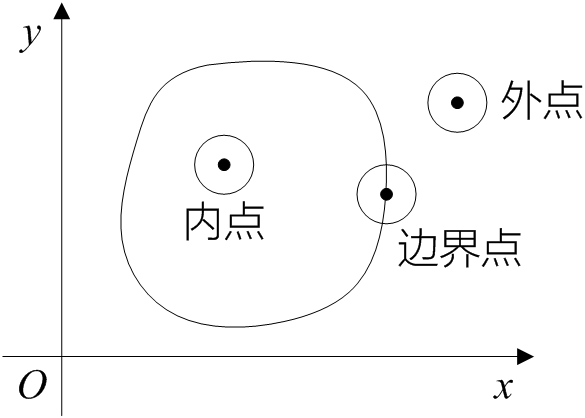
\includegraphics[height=3cm]{6.1.png}
\end{figure}

若$D$中每一个聚点都属于$D$,则称$D$为{\bf 闭集}。
若$D$中每个点都只是内点,称$D$为{\bf 开集}。
若开集$D$中任何两点均可用一条折线相连,则称为{\bf 连通的开集}或{\bf 开区域}。
开区域连同其边界称为{\bf 闭区域}。
对于点集$D$,若存在$M>0$,使得中任意两点的距离都小于$M$,称$D$为{\bf 有界区域},否则称为{\bf 无界区域}。
\end{definition}

这里,通过邻域的概念完整地定义了内点和外点,同时定义了边界点。
注意邻域概念的运用,对于内点外点,强调存在性,对于边界点,强调任一性。

最终要定义的是开区域和闭区域,类似一元函数中的开区间和闭区间,为此,需要首先定义各类点的概念和开集、闭集。

%============================================================
\subsection{二元数量值函数和二元向量值函数}

\begin{definition}[二元数量值函数]
设$D$为$\mathbb{R} ^2$的一个非空子集,$f$为$D\mapsto \mathbb{R} $的一个映射,对于$D$中的每一个矢量$\boldsymbol{p}$,$\mathbb{R} $中都有唯一的实数$z$与之对应,则称$f$为定义在$D$上的{\bf 二元数量值函数},也称{\bf 二元函数},写作:
\[
z=f\left( \boldsymbol{p} \right) \quad \boldsymbol{p}\in D
\]
其中$\boldsymbol{p}$称为{\bf 自变量},$z$称为{\bf 因变量},$D$称为{\bf 定义域}。
\end{definition}

二元数量值函数描述的是一个有序实数对到一个实数的映射:
\[
f:\boldsymbol{p}\mapsto z
\]
几何上可以用{\it xyz}直角坐标系描述。
$\boldsymbol{p}$表示平面{\it xy}平面上的点,$z$表示{\it z}轴上的值,$z=f\left( \boldsymbol{p} \right) $表示三维空间内的一个曲面。

\begin{definition}[二元向量值函数]
设$D$为$\mathbb{R} ^2$的一个非空子集,$\boldsymbol{f}$为$D\mapsto \mathbb{R} $的一个映射,对于$D$中的每一个矢量$\boldsymbol{p}$,$\mathbb{R} ^2$中都有唯一的实数$\boldsymbol{z}$与之对应,则称$\boldsymbol{f}$为定义在$D$上的{\bf 二元向量值函数},写作:
\[
\boldsymbol{z}=\boldsymbol{f}\left( \boldsymbol{p} \right) =\left( \begin{array}{c}
	P\left( \boldsymbol{p} \right)\\
	Q\left( \boldsymbol{p} \right)\\
\end{array} \right) \qquad \boldsymbol{p}\in D
\]
其中$\boldsymbol{p}$称为{\bf 自变量},$\boldsymbol{z}$称为{\bf 因变量},$D$称为{\bf 定义域},$P,Q$为$\boldsymbol{f}$对应的两个二元数量值函数。
\end{definition}

二元向量值函数描述的是一个有序实数到另一个有序实数对的映射:
\[
\boldsymbol{f}:\boldsymbol{p}\mapsto \boldsymbol{z}
\]
几何上比较难描述。

同样,可定义三维的向量值函数:
\[
\boldsymbol{z}=\boldsymbol{f}\left( \boldsymbol{p} \right) =\left( \begin{array}{c}
	P\left( \boldsymbol{p} \right)\\
	Q\left( \boldsymbol{p} \right)\\
	R\left( \boldsymbol{p} \right)\\
\end{array} \right) \qquad \boldsymbol{p}\in \mathbb{R} ^3
\]

%============================================================
\subsection{还是要光滑的}

一元函数微积分中,我们贯穿始终地考察光滑的曲线,二元函数也是一样。

学习二元函数微积分,我们可以将其与三维空间对应起来,用三维空间中的面和线,从几何角度理解二元函数微积分。
二元函数中我们喜欢的是光滑的面和线,同样需要对光滑进行定义。






\newpage
\section{极限}

本节讨论二元函数的极限。

本节要点:
\begin{itemize}
    \item 掌握极限的概念;
    \item 理解二元函数极限存在的要求。
\end{itemize}

%============================================================
\subsection{极限的概念}

\begin{definition}[极限]
设$z=f\left( \boldsymbol{p} \right) $为定义在$D$上的一个二元数量值函数,$\boldsymbol{p}_0$为$D$的聚点,如果对于$\forall \varepsilon >0$总存在$\delta >0$,使得当$0<\left\| \boldsymbol{p}-\boldsymbol{p}_0 \right\| <\delta $时,有$\left| z-A \right|<\varepsilon $,则称$A$为{\bf $f\left( \boldsymbol{p} \right) $当$\boldsymbol{p}\rightarrow \boldsymbol{p}_0$时的极限},记作$\underset{\boldsymbol{p}\rightarrow \boldsymbol{p}_0}{\lim}f\left( \boldsymbol{p} \right) $,即:
\[
\underset{\boldsymbol{p}\rightarrow \boldsymbol{p}_0}{\lim}f\left( \boldsymbol{p} \right) :=A
\]
\end{definition}

也即,对于无论什么给定多么小的$\varepsilon $,总能找到$\boldsymbol{p}_0$的一个去心邻域,使得该去心邻域内的所有矢量的函数值$z$和$A$的距离小于$\varepsilon $。
注意,这里必须是“去心”邻域。

%============================================================
\subsection{极限存在性的讨论}

二元函数中对于极限的要求是趋近方式(或称趋近方向)的任意性和趋近值的唯一性。
只要任何一条不满足,就不能说极限存在。
趋近方式的任意性要求,一般可以令$y=kx,k\in \mathbb{R} $或$y=k$或$x=k$,带入原式后简化看极限是否唯一,如果结果和$k$无关,说明满足趋近方式任意性。

这点同一元函数。
在一元函数中,左右极限均存在且相等$\Leftrightarrow $极限存在。
只是在二元函数中,“左右”两个方向变得复杂,变成了各个方向。

~

\begin{example}
设$\boldsymbol{p}=\left( x\,\,y \right) ^T$,若二元函数$f\left( \boldsymbol{p} \right) =\frac{xy}{x^2+y^2}$,讨论在原点处的极限是否存在。
\end{example}

解:

令$y=kx,k\in \mathbb{R} $表示任意方向,有:
\[
f\left( x,y \right) =\frac{kx^2}{x^2+k^2x^2}=\frac{k}{1+k^2}
\]
可见,不同的方向有不同的函数值,该二元函数在原点处不存在极限,该二元函数的图像:

\begin{figure}[ht]
\centering
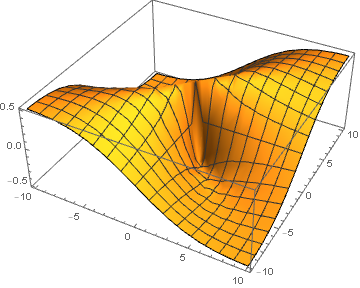
\includegraphics[height=4cm]{6.2.png}
\end{figure}

~

\begin{example}
设$\boldsymbol{p}=\left( x\,\,y \right) ^T$,若二元函数$f\left( \boldsymbol{p} \right) =\left( x^2+y^2 \right) e^{-\left( x^2+y^2 \right)}$,讨论在点$\left( -\infty ,+\infty \right) $处的极限是否存在。
\end{example}

解:

解法一,令$y=kx$表示任意方向,有:
\begin{align*}
    \underset{x\rightarrow -\infty ,y\rightarrow +\infty}{\lim}f\left( x,y \right) &=\underset{x\rightarrow -\infty ,y\rightarrow +\infty}{\lim}\left( x^2+k^2x^2 \right) e^{-\left( x^2+k^2x^2 \right)} \\
    &=\underset{x\rightarrow -\infty ,y\rightarrow +\infty}{\lim}\frac{\left( 1+k^2 \right) x^2}{e^{\left( 1+k^2 \right) x^2}} \\
    &=\underset{x\rightarrow -\infty ,y\rightarrow +\infty}{\lim}\frac{1}{e^{\left( 1+k^2 \right) x^2}} \\
    &=0
\end{align*}
极限存在且等于0。

解法二,点$\left( -\infty ,+\infty \right) $即为$\left\| \boldsymbol{p} \right\| \rightarrow \infty $:
\begin{align*}
&f\left( \boldsymbol{p} \right) =\left( x^2+y^2 \right) e^{-\left( x^2+y^2 \right)}=\left\| \boldsymbol{p} \right\| ^2e^{-\left\| \boldsymbol{p} \right\| ^2} \\
&\underset{\left\| \boldsymbol{p} \right\| ^2\rightarrow +\infty}{\lim}f\left( \boldsymbol{p} \right) =\underset{\left\| \boldsymbol{p} \right\| ^2\rightarrow +\infty}{\lim}\left\| \boldsymbol{p} \right\| ^2e^{-\left\| \boldsymbol{p} \right\| ^2}=0
\end{align*}






\newpage
\section{光滑曲面的第一个要求}

对于一个好的二元函数,我们的要求依然是“光滑”,同样要不断不折。

我们依然通过连续定义光滑的第一个要求——不断。
但是二元函数里,曲面的断复杂许多,其复杂性体现在方向的多元化。






\newpage
\section{连续}

本节讨论二元函数的连续。

本节要点:
\begin{itemize}
    \item 掌握连续的概念;
    \item 理解关于连续的定理和推论。
\end{itemize}

%============================================================
\subsection{连续的概念}

\begin{definition}[连续]
设二元数量值函数$z=f\left( \boldsymbol{p} \right) $的定义域为$D$,$\boldsymbol{p}_0$为$D$的聚点,且$\boldsymbol{p}_0\in D$,若满足
\[
\underset{\boldsymbol{p}\rightarrow \boldsymbol{p}_0}{\lim}f\left( \boldsymbol{p} \right) =f\left( \boldsymbol{p}_0 \right)
\]
则称{\bf $z=f\left( \boldsymbol{p} \right) $在$\boldsymbol{p}_0$处连续}。
反之,则称{\bf $z=f\left( \boldsymbol{p} \right) $在$\boldsymbol{p}_0$处不连续}。
不连续的点称为{\bf 间断点}。二元函数的间断点可以是孤立的点,也可以是一条或多条曲线。
\end{definition}

连续在数学上规范了什么是“不断”。
这个断不再是一元函数中简单的断点,而是需要各个方向看来不断。
虽然连续的定义从文字上和一元函数一样,但是具体判断起来要复杂得多。

%============================================================
\subsection{连续的定理}

\begin{theorem}[初等函数连续定理]
初等函数是指由常量及基本初等函数经过有限次四则运算与复合且能用一个式子表示的函数,一切二元初等函数在其定义区域内是连续的。
因此二元初等函数在其定义区域内的极限值就等于其函数值。
\end{theorem}

\begin{theorem}[最值定理]
若$z=f\left( \boldsymbol{p} \right) $在有界闭区域$D$连续,则必在$D$上有最大值和最小值。
\end{theorem}

\begin{theorem}[介值定理]
若$z=f\left( \boldsymbol{p} \right) $在有界闭区域$D$连续,且$f\left( \boldsymbol{p}_1 \right) \ne f\left( \boldsymbol{p}_2 \right) $,则对于$\forall \mu \in \left[ f\left( \boldsymbol{p}_1 \right) ,f\left( \boldsymbol{p}_2 \right) \right] $,必有$\boldsymbol{q}\in D$,使得$f\left( \boldsymbol{q} \right) =\mu $。
\end{theorem}

\begin{corollary}
若$z=f\left( \boldsymbol{p} \right) $在有界闭区域$D$连续,且有最大值和最小值$m,M$,则对于$\forall \mu \in \left[ M,m \right] $,必有$\boldsymbol{q}\in D$,使得$f\left( \boldsymbol{q} \right) =\mu $。
\end{corollary}

最值定理表达的是在有界闭区域连续的曲面必有界。
介值定理及其推论表达的是连续曲面任意两点间必有通路。






\newpage
\section{本章小结}

本章以二元函数为例讨论多元微积分的基础概念。
极限和连续的概念在二元函数均有所扩展。

要注意,极限在二元函数中比在一元函数中复杂很多。
一元函数中,极限存在的充分必要条件是左右极限都存在且相等。
二元函数中可以说类似,但要求的是各个方向的极限都存在且相等,这使得判断复杂很多,也困难很多。
连续的数学意义在于计算初等函数的极限,即,只要一个二元函数是“初等函数”,则在其定义域内任何点的极限都存在,都为该点的函数值。
注意,$f\left( \boldsymbol{p} \right) =\frac{xy}{x^2+y^2}$这种不是二元初等函数!

形而上来讲,我们开始了对高维空间几何体的“光滑”的考察。
本章是第一步,不断。






\newpage
\section{习题}

\begin{exercise}
计算下列极限:
\begin{enumerate}
    \item $\underset{x\rightarrow a,y\rightarrow 0}{\lim}\frac{\sin xy}{y}$
    \item $\underset{x,y\rightarrow 0}{\lim}\frac{x^2-y^2}{\sqrt{x-y+9}-3}$
    \item $\underset{x,y\rightarrow 0}{\lim}\frac{\ln \left[ 1+x\left( x^2+y^2 \right) \right]}{x^2+y^2}$
    \item $\underset{x,y\rightarrow 1/2}{\lim}\frac{\sin \left( x^2+2xy+y^2-1 \right)}{x+y-1}$
    \item $\underset{x\rightarrow 0,y\rightarrow 2}{\lim}\left( 1+xy \right) ^{\frac{1}{x}}$
    \item $\underset{x,y\rightarrow 0}{\lim}\left( x^2+y^2 \right) \sin \frac{1}{xy}$
    \item $\underset{x,y\rightarrow +\infty }{\lim}\left( x^2+y^2 \right) e^{-\left( x+y \right)}$
\end{enumerate}
\end{exercise}

解:

1.
\[
\underset{x\rightarrow a,y\rightarrow 0}{\lim}\frac{\sin xy}{y}=\underset{x\rightarrow a,y\rightarrow 0}{\lim}\frac{x\sin xy}{xy}=\underset{x\rightarrow a}{\lim}x=a
\]

2.
\begin{align*}
\underset{x,y\rightarrow 0}{\lim}\frac{x^2-y^2}{\sqrt{x-y+9}-3}&=\underset{x,y\rightarrow 0}{\lim}\frac{\left( x^2-y^2 \right) \cdot \left( \sqrt{x-y+9}+3 \right)}{x-y} \\
&=\underset{x,y\rightarrow 0}{\lim}\left( x+y \right) \cdot \left( \sqrt{x-y+9}+3 \right) =0
\end{align*}

3.
\begin{align*}
\underset{x,y\rightarrow 0}{\lim}\frac{\ln \left[ 1+x\left( x^2+y^2 \right) \right]}{x^2+y^2}&=\underset{x,y\rightarrow 0}{\lim}\ln \left[ 1+x\left( x^2+y^2 \right) \right] ^{\frac{1}{x^2+y^2}} \\
&=\underset{x,y\rightarrow 0}{\lim}\ln \left[ 1+x\left( x^2+y^2 \right) \right] ^{\frac{x}{x\left( x^2+y^2 \right)}} \\
&=\underset{x,y\rightarrow 0}{\lim}\ln e^x=\ln e^0=0
\end{align*}

4.
\begin{align*}
\underset{x,y\rightarrow 1/2}{\lim}\frac{\sin \left( x^2+2xy+y^2-1 \right)}{x+y-1}&=\underset{x,y\rightarrow 1/2}{\lim}\frac{\sin \left[ \left( x+y \right) ^2-1 \right]}{x+y-1} \\
&=\underset{u\rightarrow 1}{\lim}\frac{\sin \left( u^2-1 \right)}{u-1} \\
&=\underset{u\rightarrow 1}{\lim}\frac{\left( u+1 \right) \sin \left( u^2-1 \right)}{u^2-1}=2
\end{align*}

5.
\[
\underset{x\rightarrow 0,y\rightarrow 2}{\lim}\left( 1+xy \right) ^{\frac{1}{x}}=\underset{x\rightarrow 0,y\rightarrow 2}{\lim}\left( 1+xy \right) ^{\frac{y}{xy}}=\underset{y\rightarrow 2}{\lim}e^y=e^2
\]

6. 夹逼定理:
\begin{align*}
&\because -\left( x^2+y^2 \right) \leqslant \left( x^2+y^2 \right) \sin \frac{1}{xy}\leqslant x^2+y^2 \\
&\because \underset{x,y\rightarrow 0}{\lim}-\left( x^2+y^2 \right) =\underset{x,y\rightarrow 0}{\lim}\left( x^2+y^2 \right) =0 \\
&\therefore \underset{x,y\rightarrow 0}{\lim}\left( x^2+y^2 \right) \sin \frac{1}{xy}=0
\end{align*}

7. 夹逼定理:
\begin{align*}
&\because \left( x+y \right) e^{-\left( x+y \right)}<\left( x^2+y^2 \right) e^{-\left( x+y \right)}\leqslant \left( x+y \right) ^2e^{-\left( x+y \right)} \\
&\because \underset{x,y\rightarrow +\infty }{\lim}\left( x+y \right) e^{-\left( x+y \right)}=\underset{x,y\rightarrow +\infty }{\lim}\left( x+y \right) ^2e^{-\left( x+y \right)}=0 \\
&\therefore \underset{x,y\rightarrow +\infty }{\lim}\left( x^2+y^2 \right) e^{-\left( x+y \right)}=0
\end{align*}

\begin{tcolorbox}
本题总体思路是找到$x,y$的关系。
\end{tcolorbox}

~

\begin{exercise}
讨论下列函数在原点处的连续性:
\begin{enumerate}
    \item 
    $
    f\left( x,y \right) =\begin{cases}
        x\sin \frac{1}{x^2+y^2} & \left( x,y \right) \ne \left( 0,0 \right)\\
        0                       & \left( x,y \right) =\left( 0,0 \right)\\
    \end{cases}
    $
    \item 
    $
    f\left( x,y \right) =\begin{cases}
        \left( 1+x \right) ^{\frac{y}{x}} & x\ne 0\\
        e^y                               & x=0\\
    \end{cases}
    $
    \item 
    $
    f\left( x,y \right) =\begin{cases}
        \frac{x^2y}{x^4+y^2} & x^4+y^2\ne 0\\
        0                    & x^4+y^2=0\\
    \end{cases}
    $
\end{enumerate}
\end{exercise}

解:

1. 夹逼定理:
\begin{align*}
&\because -x<x\sin \frac{1}{x^2+y^2}\leqslant x \\
&\because \underset{x,y\rightarrow 0}{\lim}\left( -x \right) =\underset{x,y\rightarrow 0}{\lim}x=0 \\
&\therefore \underset{x,y\rightarrow 0}{\lim}x\sin \frac{1}{x^2+y^2}=0
\end{align*}

函数在原点处连续。

2.
\[
\underset{x,y\rightarrow 0}{\lim}\left( 1+x \right) ^{\frac{y}{x}}=\underset{y\rightarrow 0}{\lim}e^y
\]

函数在原点处连续。

3.
\[
\underset{x,y\rightarrow 0}{\lim}\frac{x^2y}{x^4+y^2}\overset{y=kx^2}{=}\underset{x\rightarrow 0}{\lim}\frac{kx^4}{x^4\left( 1+k \right)}
\]

极限不存在,所以函数在原点处不连续。

\begin{tcolorbox}
本题总体思路是计算原点处的极限。
\end{tcolorbox}









